\documentclass[12pt]{article} % use larger type; default would be 10pt
\usepackage[czech]{babel}
\usepackage[utf8]{inputenc} % set input encoding (not needed with XeLaTeX)

%%% PAGE DIMENSIONS
\usepackage{geometry} % to change the page dimensions
% \usepackage[left=2cm,right=2cm,top=2cm,bottom=2cm]{geometry}
\geometry{a4paper}
% \geometry{margin=2in} % for example, change the margins to 2 inches all round
% \geometry{landscape} % set up the page for landscape

\usepackage{graphicx} % support the \includegraphics command and options
\usepackage{wrapfig} % support the wrapfigure section

\usepackage{hyperref} % links in \tableofcontents
\hypersetup{
	colorlinks,
	citecolor=black,
	filecolor=black,
	linkcolor=black,
	urlcolor=black
}

% \usepackage[parfill]{parskip} % Activate to begin paragraphs with an empty line rather than an indent

%%% PACKAGES
\usepackage{booktabs} % for much better looking tables
\usepackage{array} % for better arrays (eg matrices) in maths
%\usepackage{paralist} % very flexible & customisable lists (eg. enumerate/itemize, etc.)
\usepackage{verbatim} % adds environment for commenting out blocks of text & for better verbatim
\usepackage{subfig} % make it possible to include more than one captioned figure/table in a single float
% These packages are all incorporated in the memoir class to one degree or another...
\usepackage{tikz} % graphs
\usepackage{pgfplots}
\usepackage{float}

%%% HEADERS & FOOTERS
\usepackage{fancyhdr} % This should be set AFTER setting up the page geometry
\pagestyle{fancy} % options: empty , plain , fancy
\renewcommand{\headrulewidth}{0pt} % customise the layout...
\lhead{}\chead{}\rhead{}
\lfoot{}\cfoot{\thepage}\rfoot{}

%%% SECTION TITLE APPEARANCE
\usepackage{sectsty}
\allsectionsfont{\sffamily\mdseries\upshape} % (See the fntguide.pdf for font help)
% (This matches ConTeXt defaults)

%%% ToC (table of contents) APPEARANCE
\usepackage[nottoc,notlof,notlot]{tocbibind} % Put the bibliography in the ToC
\usepackage[titles,subfigure]{tocloft} % Alter the style of the Table of Contents
\renewcommand{\cftsecfont}{\rmfamily\mdseries\upshape}
\renewcommand{\cftsecpagefont}{\rmfamily\mdseries\upshape} % No bold!
\newcommand{\bigsize}{\fontsize{35pt}{20pt}\selectfont}

%%% END Article customizations

\begin{document}
\begin{titlepage}
	
\includegraphics[scale=0.7]{logo.jpg}
	\vspace*{\fill}
	\begin{center}
		\textsc{\LARGE Katedra technologií a měření}\\[0.3cm]
		\textsc{\LARGE \bigsize Fyzikální elektronika}\\[0.3cm]
		\textsc{\LARGE Měření optoelektronických součástek}\\[1cm]
		Martin Zlámal \\
		Josef Sedlák \\[1cm]
		{\small\em \ Datum měření 11. listopad 2013 } \\
		{\small\em \copyright \ Datum poslední revize \today } \\
		\LaTeX
	\end{center}
	\vspace*{\fill}
\end{titlepage}
\tableofcontents
\listoffigures
\listoftables
\newpage

\section{Schéma zapojení}
\begin{figure}[H]
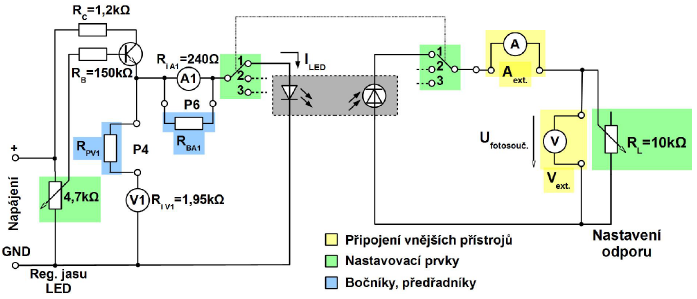
\includegraphics[scale=0.8]{schema.png}
\caption{Schéma zapojení pro měření v aktivním režimu}
\end{figure}
\begin{figure}[H]
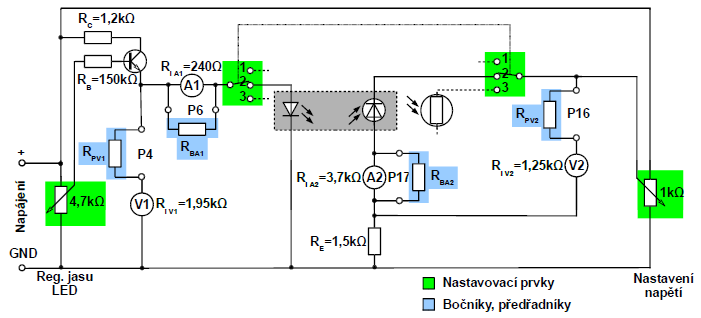
\includegraphics[scale=0.8]{schema2.png}
\caption{Schéma zapojení pro měření v pasivním režimu}
\end{figure}

\section{Katalogové parametry měřených součástek}
\begin{table}[H]
\caption{Katalogové parametry použitých součástek}
\begin{tabular}{|c|c|c|c|}
\hline 
• & fotodioda BP104 & LED červená & LED infračervená \\
\hline 
Závěrné napětí $U_R$ & $60\,V$ & $5\,V$ & $5\,V$ \\ 
\hline 
Prahové napětí $U_F$ & $350\,mV$ & $1,85\,V$ & $1,2\,V$ \\
\hline 
\end{tabular} 
\end{table}
* platné při teplotě $25^{\circ}C$

\section{Naměřené a vypočtené hodnoty}

Pro osvětlenost $0,035\,lx$ bylo nastaveno $11,5$ dílku a pro $0,07\,lx$ bylo nastaveno $21$ dílků na stupnici ampérmetru A2.

\begin{table}[H]
\caption{Naměřené hodnoty pro aktivní režim fotodiody}
\begin{tabular}{|c|c|c|c|}
\hline 
\multicolumn{2}{|c|}{Osvětlenost = 0,035 lx} & \multicolumn{2}{|c|}{Osvětlenost = 0,07 lx} \\ 
\hline 
$U_2 [mV]$ & $I_2 [uA]$ & $U_2 [mV]$ & $I_2 [uA]$ \\ 
\hline 
2,8 & 55,7 & 8,9 & 110,4 \\ 
\hline 
15,0 & 54,3 & 27,7 & 110,3 \\ 
\hline 
26,9 & 56,8 & 70,3 & 110,1 \\ 
\hline 
40,9 & 56,8 & 110,2 & 109,8 \\ 
\hline 
65,6 & 56,8 & 148,1 & 108,8 \\ 
\hline 
103,3 & 56,7 & 190,4 & 105,5 \\ 
\hline 
124,7 & 56,6 & 200,0 & 104,0 \\ 
\hline 
158,5 & 56,4 & 231,0 & 97,9 \\ 
\hline 
189,8 & 56,0 & 255,0 & 91,5 \\ 
\hline 
229,0 & 54,2 & 284,0 & 81,2 \\ 
\hline 
255,0 & 51,5 & 617,0 & 66,4 \\ 
\hline 
284,0 & 46,4 & 332,0 & 58,7 \\ 
\hline 
315,0 & 38,0 & 362,0 & 42,5 \\ 
\hline 
\end{tabular} 
\end{table}

Kde konstanta ampérmetru $A1 = A2$:
\begin{equation}
k_{AB} = \frac{n\cdot rozsah}{\alpha_{max}} = \frac{\frac{131}{11}\cdot 1}{25} = 0,476 \, mA/d
\end{equation}
S tím, že $n = R_B$:
\begin{equation}
R_B = R_{iA}\cdot \frac{1}{n-1} = 240\cdot \frac{1}{n-1} = 22 \Rightarrow n = \frac{131}{11}
\end{equation}
Obdobně konstanta voltmetru $V1$:
\begin{equation}
k_{VP} = \frac{n\cdot rozsah}{\alpha_{max}} = 1 \, mV/d
\end{equation}
S tím, že $n = R_P$:
\begin{equation}
R_P = R_{iV}\cdot (n-1) = 1950\cdot (n-1) = 0 \Rightarrow n = 1
\end{equation}
Pro výpočet výkonu musíme volit takový pracovní bod, aby byla plocha pod křivkou ve čtvrtém kvadrantu co největší. Proto volím pro osvětlení $0,07\,lx$ napětí $U = 255\,mV$ a k tomu náležící $I = 91,5\,uA$.
V tom případě je dodávaný výkon fotodiodou:
\begin{equation}
P = 255 \cdot 0,0915 = 23,33\,mW
\end{equation}
Obdobně pak výpočet výkonu pro osvětlenost $0,035\,lx$:
\begin{equation}
P = 255 \cdot 0,0515 = 13,13\,mW
\end{equation}

\begin{table}[H]
\caption{Pasivní režim fotodiody}
\begin{tabular}{|c|c|c|c|c|c|c|c|}
\hline 
\multicolumn{4}{|c|}{Osvětlenost = 0,035 lx} & \multicolumn{4}{|c|}{Osvětlenost = 0,07 lx} \\ 
\hline 
$U_2 [d]$ & $I_2 [d]$ & $U_2 [mV]$ & $I_2 [uA]$ & $U_2 [d]$ & $I_2 [d]$ & $U_2 [mV]$ & $I_2 [uA]$ \\ 
\hline 
0 & 10,5 & 0 & 49 & 0 & 23,0 & 0 & 109 \\ 
\hline 
2,5 & 10,5 & 2,5 & 49 & 2,5 & 23,5 & 2,5 & 111 \\ 
\hline 
5,0 & 10,6 & 5,0 & 50 & 5,0 & 23,6 & 5,0 & 112 \\ 
\hline 
7,5 & 10,6 & 7,5 & 50 & 7,5 & 23,6 & 7,5 & 112 \\ 
\hline 
10,0 & 10,7 & 10,0 & 51 & 10,0 & 23,7 & 10,0 & 113 \\ 
\hline 
12,5 & 10,7 & 12,5 & 51 & 12,5 & 23,7 & 12,5 & 113 \\ 
\hline 
15,0 & 10,8 & 15,0 & 51,4 & 15,0 & 23,8 & 15,0 & 113 \\ 
\hline 
17,5 & 10,8 & 17,5 & 51,4 & 17,5 & 23,8 & 17,5 & 113 \\ 
\hline 
20,0 & 10,9 & 20,0 & 52 & 20,0 & 23,9 & 20,0 & 114 \\ 
\hline 
22,5 & 10,9 & 22,5 & 52 & 22,5 & 23,9 & 22,5 & 114 \\ 
\hline 
25,0 & 11,0 & 25,0 & 52,4 & 25,0 & 24,0 & 25,0 & 114 \\ 
\hline 
\end{tabular} 
\end{table}

\begin{table}[H]
\caption{Pasivní režim fotorezistoru}
\begin{tabular}{|c|c|c|c|c|c|c|c|}
\hline 
\multicolumn{4}{|c|}{Osvětlenost = 20 lx} & \multicolumn{4}{|c|}{Osvětlenost = 30 lx} \\ 
\hline 
$U_2 [d]$ & $I_2 [d]$ & $U_2 [mV]$ & $I_2 [uA]$ & $U_2 [d]$ & $I_2 [d]$ & $U_2 [mV]$ & $I_2 [uA]$ \\ 
\hline 
0 & 0 & 0 & 0 & 0 & 0 & 0 & 0 \\ 
\hline 
2,5 & 1 & 2,5 & 0,48 & 2,5 & 1 & 2,5 & 0,48 \\ 
\hline 
5,0 & 1,5 & 5,0 & 0,7 & 5,0 & 2 & 5,0 & 0,9 \\ 
\hline 
7,5 & 2 & 7,5 & 0,9 & 7,5 & 3 & 7,5 & 1,43 \\ 
\hline 
10,0 & 2,5 & 10,0 & 1,2 & 10,0 & 4 & 10,0 & 1,9 \\ 
\hline 
12,5 & 3 & 12,5 & 1,43 & 12,5 & 4,5 & 12,5 & 2,14 \\ 
\hline 
15,0 & 3,5 & 15,0 & 1,7 & 15,0 & 5 & 15,0 & 2,4 \\ 
\hline 
17,5 & 4 & 17,5 & 1,9 & 17,5 & 6 & 17,5 & 2,9 \\ 
\hline 
20,0 & 4,5 & 20,0 & 2,1 & 20,0 & 7 & 20,0 & 3,3 \\ 
\hline 
22,5 & 5 & 22,5 & 2,4 & 22,5 & 8 & 22,5 & 3,8 \\ 
\hline 
25,0 & 5,5 & 25,0 & 2,6 & 25,0 & 9 & 25,0 & 4,3 \\ 
\hline 
\end{tabular} 
\end{table}

\section{Grafy}
\begin{figure}[H]
\centering
	\begin{tikzpicture}
		\begin{axis}[
			width=1\textwidth,
	      	height=0.4\textwidth,
			xlabel={$U[mV]$},
			ylabel={$I[uA]$},
			legend style={
				at={(0.85,0.05)},
				anchor=south west
			}]
			
		\addplot coordinates {
			(2.8,-55.7)
			(15.0,-54.3)
			(26.9,-56.8)
			(40.9,-56.8)
			(65.6,-56.8)
			(103.3,-56.7)
			(124.7,-56.6)
			(158.5,-56.4)
			(189.8,-56.0)
			(229,-54.2)
			(255,-51.5)
			(284,-46.4)
			(315,-38.0)
		};
		\addlegendentry{0,035 lx A}
	
		\addplot coordinates {
			(8.9,-110.4)
			(27.7,-110.3)
			(70.3,-110.1)
			(110.2,-109.8)
			(148.1,-108.8)
			(190.4,-105.5)
			(200,-104)
			(231,-97.9)
			(255,-91.5)
			(284,-81.2)
			(317,-66.4)
			(332,-58.7)
			(362,-42.5)
		};
		\addlegendentry{0,070 lx A}
		
		\addplot coordinates {
			(0,-49)
			(-2.5,-49)
			(-5,-50)
			(-7.5,-50)
			(-10,-51)
			(-12.5,-51)
			(-15,-51.4)
			(-17.5,-51.4)
			(-20,-52)
			(-22.5,-52)
			(-25,-52.4)
		};
		\addlegendentry{0,035 lx P}		
		
		\addplot coordinates {
			(0,-109)
			(-2.5,-111)
			(-5,-112)
			(-7.5,-112)
			(-10,-113)
			(-12.5,-113)
			(-15,-113)
			(-17.5,-113)
			(-20,-114)
			(-22.5,-114)
			(-25,-114)
		};
		\addlegendentry{0,070 lx P}		
		
		\end{axis}
	\end{tikzpicture}
	\caption{Voltamepérová charakterisitka fotodiody v pasivním i aktivním režimu}
\end{figure}

\begin{figure}[H]
\centering
	\begin{tikzpicture}
		\begin{axis}[
			width=1\textwidth,
	      	height=0.4\textwidth,
			xlabel={$U[mV]$},
			ylabel={$I[uA]$},
			legend style={
				at={(0.85,0.05)},
				anchor=south west
			}]
			
		\addplot coordinates {
			(0,0)
			(-2.5,-0.48)
			(-5,-0.7)
			(-7.5,-0.9)
			(-10,-1.2)
			(-12.5,-1.43)
			(-15,-1.7)
			(-17.5,-1.9)
			(-20,-2.1)
			(-22.5,-2.4)
			(-25,-2.6)
		};
		\addlegendentry{20 lx}
		
		\addplot coordinates {
			(0,0)
			(-2.5,-0.48)
			(-5,-0.9)
			(-7.5,-1.43)
			(-10,-1.9)
			(-12.5,-2.14)
			(-15,-2.4)
			(-17.5,-2.9)
			(-20,-3.3)
			(-22.5,-3.8)
			(-25,-4.3)
		};
		\addlegendentry{30 lx}
				
		\end{axis}
	\end{tikzpicture}
	\caption{Voltamepérová charakterisitka fotorezistoru v pasivním režimu}
\end{figure}

\section{Závěr}
Pracuje-li dioda ve IV. kvadrantu jedná se o režim zdroje. V tomto režimu dochází v oblasti přechodu PN k hromadění děr v oblasti P a elektronů v oblasti N. V tomto režimu se jedná o hradlovou fotodiodu. Jestliže se na svorky fotodiody připojí zátěžový rezistor $R_L$, začne procházet proud. Tento odpor musí být zvolen tak, aby byla plocha výkonu co největší. Bude tedy i největší výkon dodávaný fotodiodou, ale i účinnost dané součástky. Se vzrůstajícím osvětlením vzrůstá také maximální možný dodávaný výkon fotodiody. Maximální výkon fotodiody je pro osvětlení $0,035\,lx = 13,13\,mW$ a pro $0,07\,lx = 23,33\,mW$.

\end{document}